\documentclass[compress,color=usenames]{beamer}

\newcommand{\mytitlenbr}{1}
\newcommand{\mytitle}{Image Archive}

%\documentclass[compress,color=usenames,handout]{beamer}

%\usepackage{pgfpages}
%\pgfpagelayout{4 on 2}[a4paper,border shrink=5mm]

\usepackage{graphicx}
\usepackage{amsfonts,amssymb}
\usepackage{latexsym}
\usepackage{mdwtab}
\usepackage{xspace}
\usepackage{tikz}
\usetikzlibrary{shapes,snakes}
\usetikzlibrary{petri}

\DefineNamedColor{named}{Periwinkle}{cmyk}{0.57,0.55,0,0}
\DefineNamedColor{named}{Plum}{cmyk}{0.50,1,0,0}
\DefineNamedColor{named}{Red}{cmyk}{0,1,1,0}

\newcommand{\mH}[1]{\textcolor{Plum}{#1}}
\newcommand{\mT}[1]{\textcolor{Periwinkle}{#1}}

\newcommand{\tup}[1]{\langle #1 \rangle}

\newcommand{\dd}{{:}}
\newcommand{\I}{\mathcal{I}}
\newcommand{\csetsc}[2]{\{#1 \mid #2\}}
\newcommand{\cset}[1]{\{#1\}}

\newcommand{\CON}{\textsf{CON}\xspace}
\newcommand{\ROL}{\textsf{ROL}\xspace}
\newcommand{\IND}{\textsf{IND}\xspace}
\newcommand{\PROP}{\textsf{PROP}\xspace}
\newcommand{\lang}{\mathcal{L}\xspace}


\newcommand{\mytt}[1]{\textsf{\scriptsize{#1}}}
\newcommand{\mytts}[1]{\textsf{\scriptsize{#1}}}

%\usefonttheme{serif}

\mode<presentation>
 {
 \usetheme{lined}
 }

\setbeamertemplate{navigation symbols}{}


\newcommand{\F}{\mathop{\mathsf{F}\vphantom{a}}\nolimits}
\newcommand{\G}{\mathop{\mathsf{G}\vphantom{a}}\nolimits}
\newcommand{\X}{\mathop{\mathsf{X}\vphantom{a}}\nolimits}

\newcommand{\Blue}[1]{\textcolor{blue}{#1}}
\newcommand{\Red}[1]{\textcolor{red}{#1}}
\newcommand{\Green}[1]{\textcolor{PineGreen}{#1}}


\title[GLN y Aplicaciones]{\Huge Generaci\'on de Lenguaje Natural y Aplicaciones}
%\mH{Lecture \#\mytitlenbr:} \mytitle}

\author[Areces \& Benotti]{
 Carlos Areces y Luciana Benotti\\[1ex]
\normalsize \url{{carlos.areces, luciana.benotti}@gmail.com}}

\institute[INRIA / UNC]{
INRIA Nancy Grand Est, Nancy, France\\
Universidad Nacional de C\'ordoba, C\'ordoba, Argentina}

\date{ELiC 2010 - Buenos Aires - Argentina}

\begin{document}


\beamerdefaultoverlayspecification{}


\begin{frame}[plain]
 \titlepage
\end{frame}

\begin{frame}
%\frametitle{What This Tutorial is About}
\frametitle{De que se Trata este Curso?}

\begin{itemize}
\item Vamos a hablar de \mH{Generaci\'on Autom\'atica de Lenguaje Natural (GLN)}
\item Es decir, el \mH{dise\~no e implementaci\'on} de sistemas que 
\begin{itemize}
\item producen \mH{texto comprensible en lenguaje natural} (e.g., Castellano, 
Ingl\'es, etc.)
\item a partir de una \mH{representaci\'on no ling\"u\'istica} de informaci\'on
\item usando \mH{conocimiento} acerca del lenguaje y del dominio de aplicaci\'on.
\end{itemize}

\end{itemize}

\end{frame}

\begin{frame}
\frametitle{Objetivos del Curso}

\begin{itemize}
\item Dar un panorama amplio del \'area y de lo que es posible hacer hoy en d\'ia.
\item Introducir en detalle algunas de las t\'ecnicas (algunas b\'asicas y otras 
m\'as avanzadas) del \'area. 
\item Discutir algunos temas que son importantes para la aplicaci\'on de 
t\'ecnicas de GLN en proyectos concretos.
\end{itemize}
\end{frame}

\begin{frame}
\frametitle{Estructura del Curso}

\begin{columns}
\column{1.1\textwidth}
\begin{itemize}
\item \mH{Primera Parte}: Carlos Areces
\begin{itemize}
\item \mH{Lunes:} El Problema de Generaci\'on de Lenguaje Natural. Algunos sistemas de GNL.  GNL Pipeline. Representaci\'on de Informaci\'on e Inferencia para GLN.\pause

\item \mH{Martes:} Tree Adjoining Grammars (TAG). Interface Sint\'actica-Sem\'antica.
Realizaci\'on. Realizaci\'on via Charts. \pause

\item \mH{Mi\'ercoles:} Algoritmos de Generaci\'on de Expresiones Referenciales. Informaci\'on Proposicional vs.\ Informaci\'on Relacional. Optimizaci\'on de Algoritmos. Evaluaci\'on.\pause
\end{itemize}

\item \mH{Segunda Parte}: Luciana Benotti

\begin{itemize}
\item \mH{Jueves:} Entornos Virtuales (e.g., Second Life) y Aplicaciones (e.g., Tutoring) para Sistemas de GNL. Inferencia Orientada a Metas. Algoritmos de Planning y su uso en Entornos Virtuales.\pause

\item \mH{Viernes:} Generaci\'on de Referencias en un Entorno Virtual. Estrategias de Referencia. Supervisi\'on de la Interpretaci\'on. Evaluaci\'on.
\end{itemize}
\end{itemize}
\end{columns}
\end{frame}

\begin{frame}
\frametitle{Evaluaci\'on}

Viene en dos sabores

\begin{itemize}
\item \mH{Examen Takehome}:  Con preguntas te\'oricas y ejercicios pr\'acticos sobre los contenidos del curso. 
  Lo publicaremos a m\'as tardar el Lunes, en la p\'agina del curso.  Se resuelve en forma individual.  
  Se envia a las 15 d\'ias.   

\item \mH{Projectos de Desarrollo}: Definimos tres proyectos de desarrollo de sistemas de GNL extendiendo un baseline dado.  El framework esta en Java.  Se trabaja en grupos de dos personas. Se entregar\'a c\'odigo + documento explicando las ideas y testing. 
Se env\'ia a las 3 semanas.  

(Si hay m\'as interesados podemos definir algunos proyectos m\'as de este tipo.)

(Quiz\'as m\'as trabajo, pero viene con bonus.)
\end{itemize}
\end{frame}

\begin{frame}
\frametitle{Workshop Satelite de Iberamia}

Si los proyectos son interesantes (i.e., si funcionan!) los invitamos a una presentaci\'on 
en la sesi\'on de estudiantes  del:

\begin{center}

\includegraphics[scale=.4]{pics/pic15.jpg}
\end{center}

Si quieren charlar sobre los proyectos nos vienen a ver en cualquier recreo. 

\end{frame}

\begin{frame}
\frametitle{Lo que Veremos Hoy}

\begin{itemize}
\item  Introducci\'on a GLN 
\item  Un Caso de Estudio
\item  Las Tareas b\'asicas de GLN
\item  GLN en Ambientes Multimedia y Multimodales
\end{itemize}
\end{frame}

\begin{frame}
\frametitle{Lo que Veremos Hoy}

\begin{itemize}
\item  \mH{Introducci\'on a GLN} 
\begin{tabular}{|l}
 {\small Que es GLN?}\\
 {\small Ejemplos}\\
 {\small Aplicaciones t\'ipicas de GLN}\\
 {\small Cuando es apropiado usar GLN?}\\
 {\small La Arquitectura de un sistema de GLN}
\end{tabular}

\item  Un Caso de Estudio
\item  Las Tareas b\'asicas de GLN
\item  GLN en Ambientes Multimedia y Multimodales
\end{itemize}
\end{frame}


\begin{frame}
\frametitle{Qu\'e es GLN?}

\begin{itemize}
\item { {Natural language generation is the process of deliberately constructing a natural language text in order to meet specified communicative goals.}}\\

\hfill [McDonald 1992]\pause
\end{itemize}

\hfill
\includegraphics[scale=.1]{pics/crybaby.jpg}

\end{frame}

\begin{frame}
\frametitle{Qu\'e es GLN?}

\begin{itemize}
\item  \mH{Objetivo: }

\begin{itemize}
\item software que produce texto entendible y adecuado en lenguaje natural (e.g., Ingl\'es).
\end{itemize}

\item  \mH{Input: }
\begin{itemize}
\item Informaci\'on no ling\"u\'istica (e.g., una base de datos)
\end{itemize}

\item  \mH{Output: }
\begin{itemize}
\item documentos, reportes, explicaciones, mensajes de ayuda, etc.
\end{itemize}

\item \mH{Informaci\'on requerida: }
\begin{itemize}
\item Conocimiento del lenguaje y del dominio de aplicaci\'on
\end{itemize}
\end{itemize}

\end{frame}

\begin{frame}
\frametitle{Generaci\'on vs.\ Interpretaci\'on}

\begin{center}
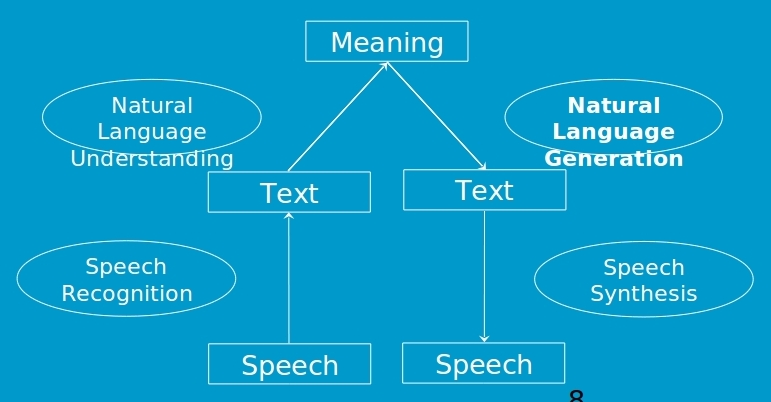
\includegraphics[scale=.4]{pics/pic1.jpg}
\end{center}
\end{frame}

\begin{frame}
\frametitle{Sistema Ejemplo \#1: FoG}

\begin{itemize}
\item \mH{Funci\'on: }
\begin{itemize}
\item Producir reportes clim\'aticos en formato texto  en Ingl\'es y en Franc\'es.
\end{itemize}
\item \mH{Input: }
\begin{itemize}
\item Im\'agen gr\'afica clim\'atica con informaci\'on num\'erica
\end{itemize}
\item \mH{Usuario: }
\begin{itemize}
\item Environment Canada (Servicio Clim\'atico Canadiense)
\end{itemize}
\item \mH{Status: }
\begin{itemize}
\item Funcionando desde 1992
\end{itemize}
\end{itemize}
\end{frame}

\begin{frame}
\frametitle{FoG: Input}

\begin{center}
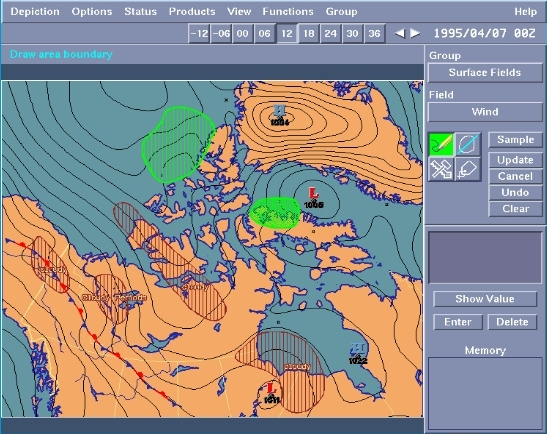
\includegraphics[scale=.4]{pics/pic2.jpg}
\end{center}

\end{frame}

\begin{frame}
\frametitle{FoG: Output}

\begin{center}
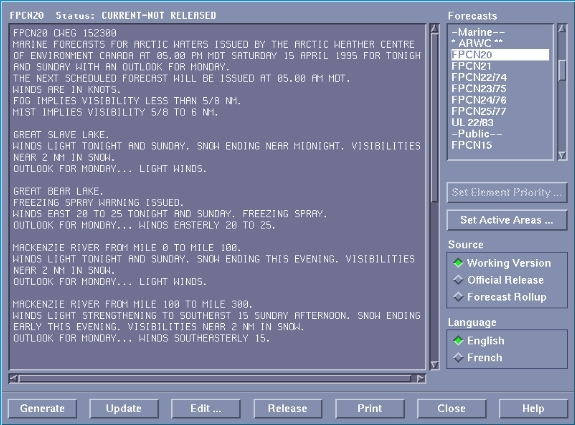
\includegraphics[scale=.4]{pics/pic3.jpg}
\end{center}

\end{frame}

\begin{frame}
\frametitle{Sistema Ejemplo \#2: PlanDoc}

\begin{itemize}
\item \mH{Funci\'on: }
\begin{itemize}
\item Producir un reporte describiendo las opciones de simulaci\'on que un ingeniero ya ha explorado
\end{itemize}
\item \mH{Input: }
\begin{itemize}
\item Un archivo de log de simulaciones
\end{itemize}
\item \mH{Usuario: }
\begin{itemize}
\item Southwestern Bell
\end{itemize}
\item \mH{Status: }
\begin{itemize}
\item Funcionando desde 1996
\end{itemize}
\end{itemize}

\end{frame}

\begin{frame}[fragile]
\frametitle{PlanDoc: Input}

\begin{verbatim}
  RUNID fiberall FIBER 6/19/93 act yes
  FA 1301 2 1995
  FA 1201 2 1995
  FA 1401 2 1995
  FA 1501 2 1995
  ANF co 1103 2 1995 48
  ANF 1201 1301 2 1995 24
  ANF 1401 1501 2 1995 24
  END. 856.0 670.2
\end{verbatim}

\end{frame}

\begin{frame}
\frametitle{PlanDoc: Output}

This saved fiber refinement includes all DLC changes in Run-ID ALLDLC. RUN-ID FIBERALL demanded that PLAN activate fiber for CSAs 1201, 1301, 1401 and 1501 in 1995 Q2. It requested the placement of a 48-fiber cable from the CO to section 1103 and the placement of 24-fiber cables from section 1201 to section 1301 and from section 1401 to section 1501 in the second quarter of 1995. For this refinement, the resulting 20 year route PWE was \$856.00K, a \$64.11K savings over the BASE plan and the resulting 5 year IFC was \$670.20K, a \$60.55K savings over the BASE plan.
\end{frame}

\begin{frame}
\frametitle{Sistema Ejemplo \#3: STOP}

\begin{itemize}
\item \mH{Function: }
\begin{itemize}
\item Producir un folleto personalizado para ayudar a dejar de fumar 
\end{itemize}
\item \mH{Input: }
\begin{itemize}
\item Questionario sobre historia, creencias, actitudes, etc.\ sobre el cigarrillo
\end{itemize}
\item \mH{Usuario: }
\begin{itemize}
\item NHS (British Health Service)
\end{itemize}
\item \mH{Status: }
\begin{itemize}
\item Utilizado por varios a\~nos
\end{itemize}
\end{itemize}

\end{frame}

\begin{frame}
\frametitle{STOP: Input}

\vspace*{-.5cm}
\begin{center}
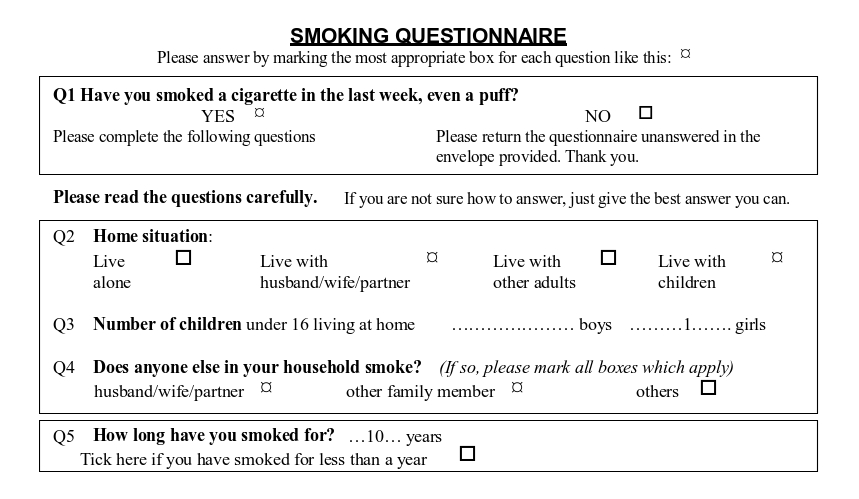
\includegraphics[scale=.5]{pics/pic4.jpg}
\end{center}

\end{frame}

\begin{frame}
\frametitle{STOP: Output}

Dear Ms Cameron\\ \ \\

 { {Thank you for taking the trouble to return the smoking questionnaire that we sent you. It appears from your answers that although you're not planning to stop smoking in the near future, you would like to stop if it was easy. You think it would be difficult to stop because \textit{smoking helps you cope with stress, it is something to do when you are bored, and smoking stops you putting on weight}. However, you have reasons to be confident of success if you did try to stop, and there are ways of coping with the difficulties. }}

\end{frame}

\begin{frame}
\frametitle{Sistema Ejemplo \#4: TEMSIS}

\begin{itemize}
\item \mH{Funci\'on: }
\begin{itemize}
\item Sumarizaci\'on de informaci\'on sobre contaminaci\'on
\end{itemize}
\item \mH{Input: }
\begin{itemize}
\item Datos ambientales + una pregunta espec\'ifica
\end{itemize}
\item \mH{Usuario: }
\begin{itemize}
\item Agencias ambientales en Francia y Alemania
\end{itemize}
\item \mH{Status: }
\begin{itemize}
\item Prototipos fueron instalados en la region Saar/Alsacia (borde entre Alemania y Francia). 
\end{itemize}
\end{itemize}

\end{frame}

\begin{frame}[fragile]
\frametitle{TEMSIS: Input Query}

\begin{verbatim}
((LANGUAGE FRENCH)
  (GRENZWERTLAND GERMANY)
  (BESTAETIGE-MS T)
  (BESTAETIGE-SS T) 
  (MESSSTATION \"Voelklingen City\"
  (DB-ID \"#2083\"
  (SCHADSTOFF \"#19\"
  (ART MAXIMUM)
  (ZEIT ((JAHR 1998)
         (MONAT 7)
         (TAG 21))))
\end{verbatim}

\end{frame}

\begin{frame}
\frametitle{TEMSIS: Output Summary}

\begin{itemize}
\item \mH{Franc\'es:}

Le 21/7/1998 \`a la station de mesure de V\"olklingen-City, la valeur moyenne maximale d'une demi-heure (Halbstundenmittelwert) pour l'ozone atteignait 104.0 $\mu$g/m${}^3$. Par cons\'equent, selon le decret MIK (MIK-Verordnung), la valeur limite autoris\'ee de 120 $\mu$g/m${}^3$ n'a pas \'et\'e d\'epass\'e.

\item \mH{Alem\'an:}

Der h\"ochste Halbstundenmittelwert f\"ur Ozon an der Me{\ss}station V\"olklingen-City erreichte 
am 21.7.1998 104.0 $\mu$g/m${}^3$, womit der gesetzlich zul\"assige Grenzwert nach MIK-Verordnung von 
120 $\mu$g/m${}^3$ nicht \"uberschritten wurde.
\end{itemize}

\end{frame}

\begin{frame}
\frametitle{Tipos de Aplicaciones de GLN}

\begin{itemize}
\item \mH{Producci\'on autom\'atica de documentos}
\begin{itemize}
\item reportes clim\'aticos, reporte de simulaciones, cartas, \ldots
\end{itemize}
\item \mH{Presentaci\'on de informaci\'on al p\'ublico en forma entendible}
\begin{itemize}
\item imformes m\'edicos, sistemas expertos de inferencia, \ldots
\end{itemize}
\item \mH{Ense\~nanza}
\begin{itemize}
\item educaci\'on a distancia
\end{itemize}
\item \mH{Entretenimiento/Arte}
\begin{itemize}
\item bromas (?), historias (??), poes\'ia (???)
\end{itemize}
\end{itemize}

\end{frame}

\begin{frame}
\frametitle{El Rol de la Computadora}

 Dos posibilidades
\begin{itemize}
\item  El sistema produce un documento \mH{autom\'aticamente} (sin ayuda humana) 

 reportes clim\'aticos, reportes de simulaciones, cartas a pacientes,
 res\'umenes de datos estad\'isticos, explicaciones en sistemas expertos.

\item El sistema \mH{ayuda a un redactor humano} a crear un documento:

 reportes clim\'aticos, reportes de simulaciones, cartas a pacientes,
 pedidos de patentes, documentos t\'ecnicos (manuales), pedidos de empleo
\end{itemize}

\end{frame}

\begin{frame}
\frametitle{En qu\'e Casos son las T\'ecnicas de GLN Adecuadas?}

Opciones a Considerar:

\begin{itemize}
\item { \mH{Texto vs.\ Gr\'aficos}}
\begin{itemize}
\item Qu\'e medio es mejor?
\end{itemize}
\item { \mH{Generaci\'on Autom\'atica vs. Autor\'ia Humana}}
\begin{itemize}
\item Son los datos necesarios accesibles? 
\item Vale la pena (e.g., econ\'omicamente)?
\end{itemize}
\item { \mH{GLN vs.\ Concatenaci\'on de strings}}
\begin{itemize}
\item Cu\'anta variaci\'on hay en el texto?
\item Que impacto tiene la calidad gramatical del texto? 
\end{itemize}
\end{itemize}

\end{frame}

\begin{frame}
\frametitle{Calidad Gramatical}

\begin{itemize}
\item La generaci\'on de texto \mH{ling\"u\'isticamente bien formado} requiere la verificaci\'on de constraints
\begin{itemize}
\item ortogr\'aficos, morfol\'ogicos, sint\'acticos
\item referencia, elecci\'on de palabras, pragm\'aticas
\end{itemize}
\item Estos constraints se verifican \mH{autom\'aticamente} por un sistema de GLN
\begin{itemize}
\item en forma autom\'atica, el 100\% de los casos
\end{itemize}
\item Los desarrolladores de sistemas basados en concatenaci\'on de strings tienen que verificar
 el cumplimiento de estos strings \mH{manualmente y v\'ia testing}
\begin{itemize}
\item Muy trabajoso
\item Dif\'icil de garantizar exactitud del 100\%
\end{itemize}
\end{itemize}

\end{frame}

\begin{frame}
\frametitle{Ejemplo: Syntaxis, agregaci\'on}

\label{f48}
\begin{itemize}
\item { {Output de sistemas de IA Medical existentes:}}

\begin{quote}
 The primary measure you have chosen, CXR shadowing, should be justified in comparison to TLC and walking distance as my data reveals they are better overall. Here are the specific comparisons:
\medskip

 TLC has a lower patient cost TLC is more tightly distributed TLC is more objective walking distance has a lower patient cost
\end{quote}
\end{itemize}

\end{frame}

\begin{frame}
\frametitle{Ejemplo: Pragm\'atica}

\label{f50}
\begin{itemize}
\item Output de un sistema que da versiones en ingl\'es de consultas a una base de datos:

\begin{quote} 
The number of households such that there is at least 1 order with dollar amount greater 
than or equal to \$100.\pause
\end{quote}

\begin{itemize}

\item Se interpreta como ``number of households which have placed an order 
\mbox{$>=$} \$100'' \pause
\item La consulta inicial era el n\'umero total de casas en la base de datos, si habia alguna 
orden en la base de datos (de cualquier casa) por mas de \$100
\end{itemize}
\end{itemize}

\end{frame}

\begin{frame}
\frametitle{La Arquitectura de un Sistema de GLN}

\begin{itemize}
\item { {Las tareas b\'asicas en un sistema de GLN}}
\item Arquitectura de Pipeline 
\item Alternative Architectures
\end{itemize}

\end{frame}

\begin{frame}
\frametitle{Las Tareas B\'asicas en un sistema de GLN}

\begin{enumerate}
\item { { Determinaci\'on de Contenido (Content determination)}}
\item { { Estructuraci\'on del Documento (Document structuring)}}
\item { { Agregaci\'on (Aggregation)}}
\item { { Lexicalizaci\'on (Lexicalisation)}}
\item { { Generaci\'on de Expresiones Referenciales (Referring expression generation)}}
\item { { Realizaci\'on Ling\"u\'istica (Linguistic realisation)}}
\item { { Realizaci\'on de Estructura (Structure realisation}}
\end{enumerate}

\end{frame}

\begin{frame}
\frametitle{Las Tareas B\'asicas en un sistema de GLN}

\begin{center}
\begin{tabular}{|l|c|}  \hline
Content Determination & \mH{Document} \\
Document Structuring &  \mH{planning}\\ \hline
Aggregation &  \mH{Micro-}\\
Lexicalisation & \mH{planning}\\
Referring Expression Generation & \\ \hline
Linguistic Realisation & \mH{Surface}\\
Structure Realisation & \mH{realization}\\ \hline
\end{tabular}
\end{center}

\end{frame}

\begin{frame}
\frametitle{Una Arquitectura Pipeline}

\begin{center}
Document\\
planning\\
$\downarrow$\\
\mH{Document plan}\\
$\downarrow$\\
Microplanning\\
$\downarrow$\\
\mH{Text Specificacion}\\
$\downarrow$\\
Surface\\
Realization
\end{center}

\end{frame}

\begin{frame}
\frametitle{Otras Arquitecturas}

\label{f60}
\begin{itemize}
\item { {Variaciones de la \mH{arquitectura ``standard''}:}}
\begin{itemize}
\item { {Alterar el orden de las tareas}}
\item { {Permitir feedback entre las distintas etapas}}
\end{itemize}
\item { {Un sistema integrado donde \mH{todas las tareas se combinan}:}}
\begin{itemize}
\item { {representar todas las tareas en forma uniforme: e.g.\ como constraints, axiomas, operadores de planning, \ldots}}
\item { {alimentar estas especificaciones a un  constraint-solver, demostrador de teoremas, \ldots}}
\end{itemize}
\end{itemize}
\end{frame}

\begin{frame}
\frametitle{Temas de Investigaci\'on}

\label{f62}
\begin{itemize}
\item { {Cu\'ando es texto la mejor forma de cominicarse con el usuario?}}
\item { {Cu\'ando es GLN mejor que concatenaci\'on de strings?}}
\item { {Existe alguna arquitectura que combine la elegancia te\'orica y la flexibilidad de un sistema integrado, con la simplicidad de una arquitectura pipeline?}}
\item { {Como debemos representar Document Plans y Text Specifications?}}
\end{itemize}

\end{frame}

\begin{frame}
\frametitle{Lo que Veremos Hoy}

\begin{itemize}
\item  Introducci\'on a GLN 
\item  \mH{Un Caso de Estudio}
\item  Las Tareas b\'asicas de GLN
\item  GLN en Ambientes Multimedia y Multimodales
\end{itemize}
\end{frame}


\begin{frame}
\frametitle{Lo que Veremos Hoy}

\begin{itemize}
\item  Introducci\'on a GLN 
\item  \mH{Un Caso de Estudio}
\begin{tabular}{|l}
Generando Res\'umenes Clim\'aticos\\
Recopilaci\'on y Uso de Corpus\\
\end{tabular}
\item  Las Tareas b\'asicas de GLN
\item  GLN en Ambientes Multimedia y Multimodales
\end{itemize}
\end{frame}


\begin{frame}
\frametitle{Un Caso de Estudio en GLN Aplicada}

\begin{itemize}
\item Cada mes, un peri\'odico institucional publica un resumen clim\'atico del mes
\item El resumen se basa en datos meteorol\'ogicos recolectados autom\'aticamente
\item La persona que hasta el momento hac\'ia este trabajo deja la instituci\'on
\end{itemize}

\end{frame}

\begin{frame}
\frametitle{Un Resumen Clim\'atico}

\begin{center}
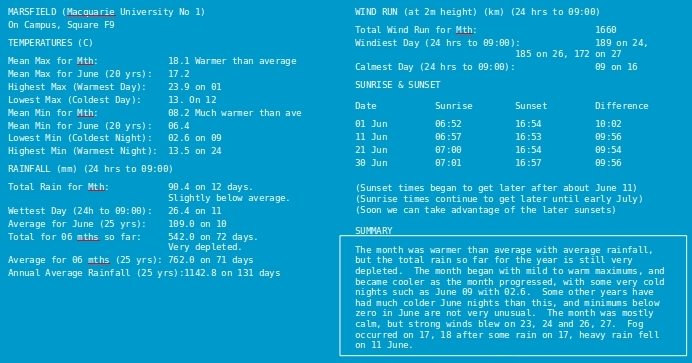
\includegraphics[scale=.47]{pics/pic5.jpg}
\end{center}

\end{frame}


\begin{frame}
\frametitle{Output: Un Resumen Clim\'atico}

\begin{quote}
\item { {The month was warmer than average with average rainfall, but the total rain so far for the year is still very depleted. The month began with mild to warm maximums, and became cooler as the month progressed, with some very cold nights such as June 09 with 02.6. Some other years have had much colder June nights than this, and minimums below zero in June are not very unusual. The month was mostly calm, but strong winds blew on 23, 24 and 26, 27. Fog occurred on 17, 18 after some rain on 17, heavy rain fell on 11 June.}}
\end{quote}

\end{frame}

\begin{frame}[fragile]
\frametitle{Los Datos de Input}

\begin{columns}
\column{1.1\textwidth}
\begin{itemize}
\item Un conjunto de \mH{16 datos recolectados autom\'aticamente cada 15 minutos}: presi\'on del aire, temperatura, velocidad del viento, lluvia ca\'ida, \ldots.
\item Preprocesados para obtener un instancia de  DailyWeatherRecords:

\begin{verbatim}
((type dailyweatherrecord)
   (date ((day ...)
          (month ...)
          (year ...)))
 (temperature ((minimum ((unit degrees-centigrade)
                         (number ...)))
               (maximum ((unit degrees-centrigrade)
                         (number ...)))))
 (rainfall ((unit millimetres)
            (number ...))))
\end{verbatim}

\end{itemize}
\end{columns}
\end{frame}

\begin{frame}
\frametitle{Otros Datos Disponibles}

\label{f74}
\begin{itemize}
\item  \mH{Datos Hist\'oricos:} E.g.\ Temperaturas m\'aximas y m\'inimas registradas para los distintos meses.

Nos permite generar cosas como ``La temperatura excedi\'o la m\'axima hist\'orica para Mayo''

\item \mH{Datos Promedio:} E.g.\ Valores promedio de temperatura y lluvia en lo que viene del a\~no.

Nos permite generar cosas como ``El mes fue m\'as c\'alido que el anterior'' 
\end{itemize}

\end{frame}

\begin{frame}
\frametitle{An\'alisis de Requirimientos basado en Corpus}

Un \mH{corpus}
\begin{itemize}
\item consiste de ejemplos de textos generados anteriormente con sus correspondientes datos de entrada

\item especifica `mediante ejemplos' la funcionalidad esperada del sistema de GLN
\item servir\'a de patr\'on para los mensajes que queremos generar 
\end{itemize}

\end{frame}

\begin{frame}
\frametitle{An\'alisis de Requirimientos basado en Corpus}

 { {Cuatro Actividades:}}
\begin{itemize}
\item \mH{recolectar un corpus inicial} de textos generados a mano con sus correspondientes datos de input

\item \mH{analizar} el contenido del corpus en termino de los datos de input
\item desarrollar un \mH{corpus target}
\item especificar formalmente el \mH{mapeo de datos a texto} 
\end{itemize}
\end{frame}

\begin{frame}
\frametitle{Paso 1: Crear el Corpus Inicial}

 Recolectar corpus de texto (generados anteriormente a mano) y los correspondientes datos de input
\begin{itemize}
\item Una fuente pueden ser ejemplos archivados 
\item Si no existen ejemplos anteriores se deber\'a recurrir a expertos del dominio para que produzcan ejemplos
\item El corpus debe proveer ejemplos de la totalidad de casos que se esperan manejar con el sistema de GLN
\end{itemize}

\end{frame}

\begin{frame}
\frametitle{Texto Inicial}

\begin{itemize}
\item { {SUMMARY}}
\item { {The month was rather dry with only three days of rain in the middle of the month. The total for the year so far is very depleted again, after almost catching up during March. Mars Creek dried up again on 30th April at the waterfall, but resumed on 1st May after light rain. This is the fourth time it dried up this year.}}
\end{itemize}

\end{frame}

\begin{frame}
\frametitle{Paso 2: Analizar el Contenido del Corpus}

\begin{itemize}
\item \mH{Objetivo:}
\begin{itemize}
\item determinar de donde viene la informaci\'on contenida en el texto, y en qu\'e medida el sistema de GLN 
tendr\'a que manipular esta informaci\'on
\end{itemize}
\item \mH{Resultado: }
\begin{itemize}
\item un entendimiento detallado de la correspondencia entre los datos de entrada existentes y el texto generado en cada caso en el corpus
\end{itemize}
\end{itemize}

En particular queremos \mH{clasificar} el texto a generar en 4 clases: Texto fijo, texto generado directamente a partir de los datos, texto generado a partir de datos computables, texto no soportado por los datos.   

\end{frame}

\begin{frame}
\frametitle{Ejemplo}

{SUMMARY}

{ {The month was rather dry with only three days of rain in the middle of the month. The total for the year so far is very depleted again, after almost catching up during March. Mars Creek dried up again on 30th April at the waterfall, but resumed on 1st May after light rain. This is the fourth time it dried up this year.}}

\end{frame}


\begin{frame}
\frametitle{Texto Fijo}

\mH{SUMMARY}

{ {The month was rather dry with only three days of rain in the middle of the month. The total for the year so far is very depleted again, after almost catching up during March. Mars Creek dried up again on 30th April at the waterfall, but resumed on 1st May after light rain. This is the fourth time it dried up this year.}}

\end{frame}

\begin{frame}
\frametitle{Obtenido  Directamente de los Datos}

SUMMARY

\mH{The month was rather dry with only three days of rain in the middle of the month}. The total for the year so far is very depleted again, after almost catching up during March. Mars Creek dried up again on 30th April at the waterfall, but resumed on 1st May after light rain. This is the fourth time it dried up this year.

\end{frame}

\begin{frame}
\frametitle{Obtenido de Datos Computables}

SUMMARY

The month was rather dry with only three days of rain in the middle of the month. \mH{The total for the year so far is very depleted again, after almost catching up during March}. Mars Creek dried up again on 30th April at the waterfall, but resumed on 1st May after light rain. This is the fourth time it dried up this year.

\end{frame}

\begin{frame}
\frametitle{Sin Datos de Soporte}

SUMMARY

The month was rather dry with only three days of rain in the middle of the month. The total for the year so far is very depleted again, after almost catching up during March. \mH{Mars Creek dried up again on 30th April at the waterfall, but resumed on 1st May after light rain. This is the fourth time it dried up this year.}

\end{frame}


\begin{frame}
\frametitle{Resolviendo el Problema de la Falta de Datos}

\begin{itemize}
\item Quizas podemos \mH{dar datos adicionales} al sistema 
    \begin{itemize}
        \item agregar censores en Mars Creek?
    \end{itemize}
\item Si el sistema en realidad esta ayudando en la redacci\'on a un humano, esta informaci\'on podr\'a ser \mH{agregada m\'as tarde}
    \begin{itemize}
    \item el sistema produce las primeras dos sentencias, el redactor humano agrega luego las \'ultimas dos     \end{itemize}
\item El corpus target es revisado para \mH{eliminar} las frases vinculadas con este tipo de informaci\'on.
    \begin{itemize}
    \item produciremos solamente las primeras dos sentencias
    \end{itemize}
\end{itemize}

\end{frame}

\begin{frame}
\frametitle{Paso 3: Construyendo el Corpus Target}

\begin{itemize}
\item { \mH{Cambios Obligatorios:}}
\begin{itemize}
\item { {eliminar texto generado a partir de datos inaccessible}}
\item { {especificar las porciones que ser\'an generadas por el redactor humano}}
\end{itemize}
\item { \mH{Cambios Opcionales:}}
\begin{itemize}
\item { {simplificar el texto para que sea m\'as f\'acil de generar}}
\item { {mejorar la coordinaci\'n entre el texto generado autom\'aticamente y el texto generado por el redactor humano}}
\end{itemize}
\end{itemize}

\end{frame}

\begin{frame}
\frametitle{Texto Target}

\begin{quote}
 { {The month was rather dry with only three days of rain in the middle of the month. The total for the year so far is very depleted again.}}
\end{quote}

\end{frame}

\begin{frame}
\frametitle{Paso 4: Especificaci\'on Funcional}

\label{f104}
\begin{itemize}
\item { {Basada en el corpus target obtenido}}
\item { {Define en forma expl\'icita el role del redactor humano (si corresponde)}}
\item { {Define en forma expl\'icita la estructura y el rango del input que ser\'a utilizado}}
\end{itemize}

\end{frame}

\begin{frame}
\frametitle{Texto Inicial vs.\ Texto Target}

\mH{Texto Initial:} The month was our driest and warmest August in our 24 year record, and our first `rainless' month. The 26th August was our warmest August day in our record with 30.1, and our first `hot' August day (30). The month forms part of our longest dry spell 47 days from 18 July to 02 September 1995. Rainfall so far is the same as at the end of July but now is very deficient.
\bigskip

\mH{Texto Target:} The month was the driest and warmest August in our 24 year record, and the first rainless month of the year. 26th August was the warmest August day in our record with 30.1, and the first hot day of the month. Rainfall for the year is now very deficient.
 \end{frame}

\begin{frame}
\frametitle{Vale la Pena usar GLN?}

\begin{itemize}
\item Para un resumen por mes probablemente no.  Sobre todo teniendo en cuanta las \mH{simplificaciones} que debimos introducir en los textos para hacerlso f\'acil de generar.

\item Pero nuestro cliente esta interesado en un caso piloto porque: 
\begin{itemize}
\item en el futuro los reportes se haran de forma \mH{semanal}. 
\item hay \mH{varios sitios} de recolecci\'on autom\'atica de datos, y el sistema podr\'ia utilizarse en todos ellos. 
\end{itemize}
\end{itemize}

\end{frame}

\begin{frame}
\frametitle{Lo que Veremos Hoy}

\begin{itemize}
\item  Introducci\'on a GLN 
\item  Un Caso de Estudio
\item  \mH{Las Tareas B\'asicas de GLN}
\item  GLN en Ambientes Multimedia y Multimodales
\end{itemize}
\end{frame}

\begin{frame}
\frametitle{Lo que Veremos Hoy}

\begin{itemize}
\item  Introducci\'on a GLN 
\item  Un Caso de Estudio
\item  \mH{Las Tareas B\'asicas de GLN}
\begin{tabular}{|l}
Document Planning\\
Microplanning\\
Surface Realization
\end{tabular}
\item  GLN en Ambientes Multimedia y Multimodales
\end{itemize}
\end{frame}

\begin{frame}
\frametitle{Inputs y Outputs}

\begin{center}
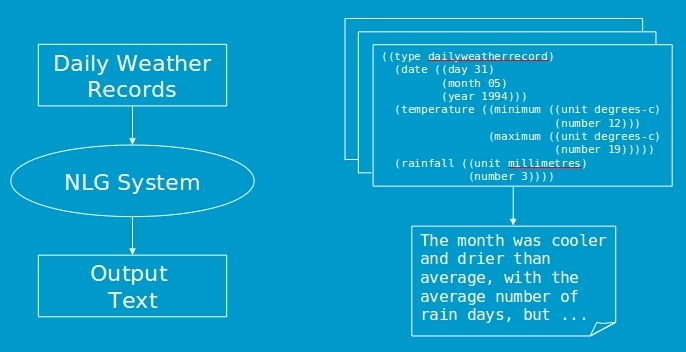
\includegraphics[scale=.4]{pics/pic6.jpg}
\end{center}

\end{frame}

\begin{frame}
\frametitle{La Arquitectura}

\begin{center}
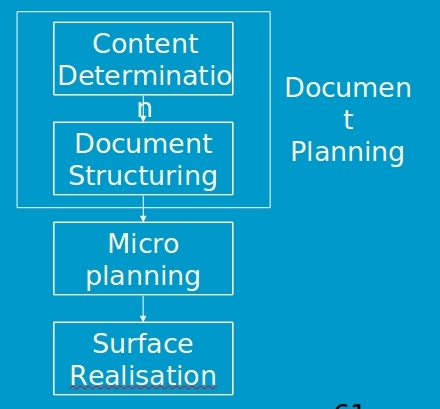
\includegraphics[scale=.4]{pics/pic7.jpg}
\end{center}
 
\end{frame}

\begin{frame}
\frametitle{Document Planning}

\begin{itemize}
\item { \mH{Objetivos: }}
\begin{itemize}
\item determinar que informaci\'on debe comunicarse
\item determinar como estructurar esta informaci\'on para obtener un texto 
coherente
\end{itemize}
\item { \mH{Existen dos enfoques usuales:}}
\begin{itemize}
\item m\'etodos basados en observaciones directas de c\'omo se estructura el texto en ejemplos
\item m\'etodos basados en razonamiento sobre coherencia del discurso y el objetivo comunicativo del texto
\end{itemize}
\end{itemize}
 
\end{frame}



\begin{frame}
\frametitle{Content Determination}

\label{f124}
\begin{itemize}
\item { {Usualmente basado en \mH{mensajes}: estructuras de informaci\'on predefinidas que}}
\begin{itemize}
\item se corresponden con bloques de informaci\'on en el texto
\item agrupan elementos de informaci\'on de forma de facilitar su expresion textual
\end{itemize}

\item { \mH{Idea Fundamental:}}
\begin{itemize}
\item A partir del an\'alisis del corpus, identificar los agrupamientos de elementos de informaci\'on lo m\'as grande posibles, que no limiten nuestra flexibilidad al querer generarlos.  
\end{itemize}
\end{itemize}
 
\end{frame}

\begin{frame}
\frametitle{Content Determination en WeatherReporter}

\begin{itemize}
\item { \mH{Mensajes Rutinarios}}

\ \ -- MonthlyRainFallMsg, 

\ \ -- MonthlyTemperatureMsg, 

\ \ -- RainSoFarMsg, 

\ \ -- MonthlyRainyDaysMsg

\item Se incluyen en todos los resumenes a generar
\end{itemize}

 
\end{frame}

\begin{frame}[fragile]
\frametitle{Content Determination en WeatherReporter}

 { {MonthlyRainfallMsg:}}
\begin{verbatim}
((message-id msg091)
 (message-type monthlyrainfall)
 (period ((month 04)
          (year 1996)))
 (absolute-or-relative relative-to-average)
 (relative-difference ((magnitude ((unit millimeters)
                                   (number 4)))
                       (direction +))))
\end{verbatim}

\end{frame}

\begin{frame}
\frametitle{Content Determination en WeatherReporter}

\begin{itemize}
\item { \mH{Mensajes de Eventos Significativos}}

\ \ \ -- RainEventMsg, 

\ \ \ -- RainSpellMsg, 

\ \ \ -- TemperatureEventMsg, 

\ \ \ -- TemperatureSpellMsg

\item S\'olo se general cuando los datos lo indiquen: e.g., si se registran lluvias en un n\'umero de d\'ias consecutivos mayor a una cantidad especificada. 
\end{itemize}
\end{frame}

\begin{frame}[fragile]
\frametitle{Content Determination en WeatherReporter}

 { {A RainSpellMsg:}}
\begin{verbatim}
((message-id msg096)
 (message-type rainspellmsg)
 (period ((begin ((day 04)
                  (month 02)
                  (year 1995)))
          (end ((day 11)
                (month 02)
                (year 1995)))
          (duration ((unit day)
                     (number 8)))))
 (amount ((unit millimetres)
          (number 120))))
\end{verbatim}
\end{frame}

\begin{frame}
\frametitle{Document Structuring mediante Esquemas}

La idea b\'asica
\begin{itemize}
\item Los textos de un determinado tipo siguen (usualmente) \mH{patrones convencionalizados} 
\item estos patrones pueden ser expresados mediante \mH{'gram\'aticas de texto'} que indican el contenido a 
generar y aseguran una estructura coherente. 
\item estos patrones especifican \mH{como se construir\'a el plan de un documento particular} usando esquemas
m\'as chicos o mensajes at\'omicos.  
\end{itemize}
\end{frame}

\begin{frame}
\frametitle{Document Structuring mediante Esquemas}

{{Implementando esquemas:}}
\begin{itemize}
\item los esquemas m\'as simples se especifican mediante gram\'aticas
\item esquemas m\'as flexibles se especifican como macros, o clases de librer\'ias sobre lenguajes de 
programaci\'on convencionales, donde cada esquema es un procedimiento. 
\item este es, hoy en d\'ia, el m\'etodo de document planning mas usual en sistemas de GLN
\end{itemize}

 
\end{frame}

\begin{frame}
\frametitle{Derivando Esquemas a Partir del un Corpus}

{ {Usando el corpus target:}}
\begin{itemize}
\item tomar un cierto n\'umero (peque\~no) de \mH{textos similares}
\item identificar los mensajes, y determinar como cada mensaje puede ser computado a partir de los datos de input
\item proponer reglas o estructuras que expliquen \mH{por que el mensaje x es en el texto A pero no en el B}. (Esta tarea puede ser m\'as f\'acil si los mensajes se organizan en una taxonom\'ia) 
\item discutir este an\'alisis con \mH{expertos del dominio}, e iterar
\item repetir los pasos anteriores con \mH{conjuntos cada vez mas grandes} de texto del corpus
\end{itemize}

\end{frame}

\begin{frame}
\frametitle{Document Structuring en WeatherReporter}

 { {Un esquema simple:}}

\begin{center} \tt
\begin{tabular}{l}
WeatherSummary $\to$\\
\ \ \ \ \  MonthlyTempMsg\\
\ \ \ \ \   MonthlyRainfallMsg\\
\ \ \ \ \   RainyDaysMsg\\
\ \ \ \ \   RainSoFarMsg\\
\end{tabular}
\end{center}

 \end{frame}

\begin{frame}
\frametitle{Document Structuring en WeatherReporter}

Un conjunto de esquemas m\'as interesante
\vspace*{-.6cm}

\begin{center}\tt
\begin{tabular}{l}
WeatherSummary $\to$      \\
\ \ \ \ TemperatureInformation RainfallInformation\\
\ \\
TemperatureInformation $\to$\\
\ \ \ \  MonthlyTempMsg [ExtremeTempInfo] [TempSpellsInfo]\\
\ \\
RainfallInformation $\to$\\
\ \ \ \  MonthlyRainfallMsg [RainyDaysInfo] [RainSpellsInfo]\\
\ \\
RainyDaysInfo $\to$\\
\ \ \ \  RainyDaysMsg [RainSoFarMsg]\\
\ldots
\end{tabular}
\end{center}

\end{frame}

\begin{frame}
\frametitle{Esquemas: Pros and Cons}

\label{f148}
\begin{itemize}
\item { \mH{Ventajas:}}
\begin{itemize}
\item Computacionalmente eficientes
\item Relativamente simples de obtener a partir de un corpus
\item Permiten especificar naturalmente particularidades de un determinado dominio (i.e., customizables)
\item Pueden ser arbitrariamente complejos 
\end{itemize}
\item { \mH{Desventajas}}
\begin{itemize}
\item { {Flexibilidad Limitada: requieren la especificaci\'on a priori de todas las estructuras posibles}}
\item { {Portabilidad Limitada: en general, son particulares al dominio}}
\end{itemize}
\end{itemize} 
\end{frame}

\begin{frame}
\frametitle{Document Structuring mediante Razonamiento Expl\'icito}

\label{f150}
\begin{itemize}
\item { \mH{Observaci\'on:}}
\begin{itemize}
\item La coherencia de un texto se obtiene a partir de ciertas relaciones que existen 
entre las distintas partes. Relaciones como secuencia narrativa, elaboraci\'on, justificaci\'on
\end{itemize}
\item { \mH{Idea:}}
\begin{itemize}
\item organizar el conocimiento de que es lo que hace un texto coherente en forma de reglas
\item usar estas reglas para construir textos din\'amicamente a partir de fragmentos elementales 
mediante razonamiento del rol de cada elemento en el texto a construir
\end{itemize}
\end{itemize}
 \end{frame}

\begin{frame}
\frametitle{Document Structuring mediante Razonamiento Expl\'icito}

\label{f152}
\begin{itemize}
\item T\'ipicamente usan tecnicas de AI planning
\begin{itemize}
\item Goal = el efecto comunicativo deseado
\item Elementos del Plan = mensajes o estructuras que combinan mensajes  (subplans)
\end{itemize}
\item Puede requerir razonamiento expl\'icito sobre el conocimiento del usuario.
\item Usualmente basados en ideas de Rethorical Structure Theory
\end{itemize}
 
\end{frame}

\begin{frame}
\frametitle{Rethorical Structure Theory}
\begin{itemize}
	
\item D1: You should come to the Northern Beaches Ballet performance on Saturday.
\item D2: The show is really good.
\item D3: It got a rave review in the Times. 
\item D4: You can get the tickets from the shop next door.
\end{itemize}
\end{frame}

\begin{frame}
\frametitle{Rethorical Structure Theory}

\begin{center}
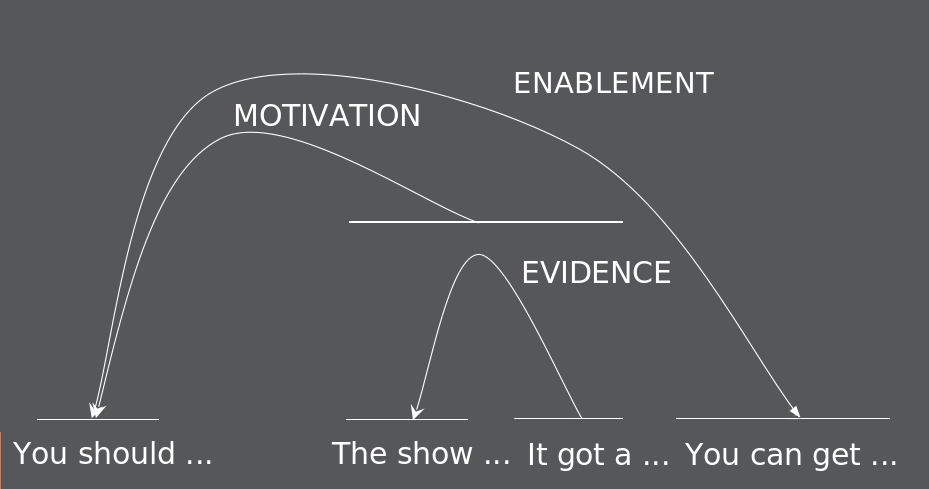
\includegraphics[scale=.47]{pics/pic8.jpg}
\end{center}

\end{frame}

\begin{frame}[fragile]
\frametitle{Definici\'on de una Relacion en RST}

\begin{verbatim}
Relation name:  Motivation

Constraints on N:
Presents an action (unrealised) in which the hearer 
is the actor

Constraints on S:
Comprehending S increases the hearer’s desire to 
perform the action presented in N

The effect:
The hearer’s desire to perform the action presented 
in N is increased
\end{verbatim}

\end{frame}


\begin{frame}
\frametitle{Document Structuring en WeatherReporter}

\begin{itemize}
\item Tres relaciones RST basicas
\begin{itemize}
\item SEQUENCE
\item ELABORATION
\item CONTRAST
\end{itemize}

\item Las reglas de aplicaci\'on de cada una de estas relaciones 
se definen a partir de atributos de los mensajes
\end{itemize}
\end{frame}

\begin{frame}
\frametitle{Atributos de Mensajes}

\begin{center}
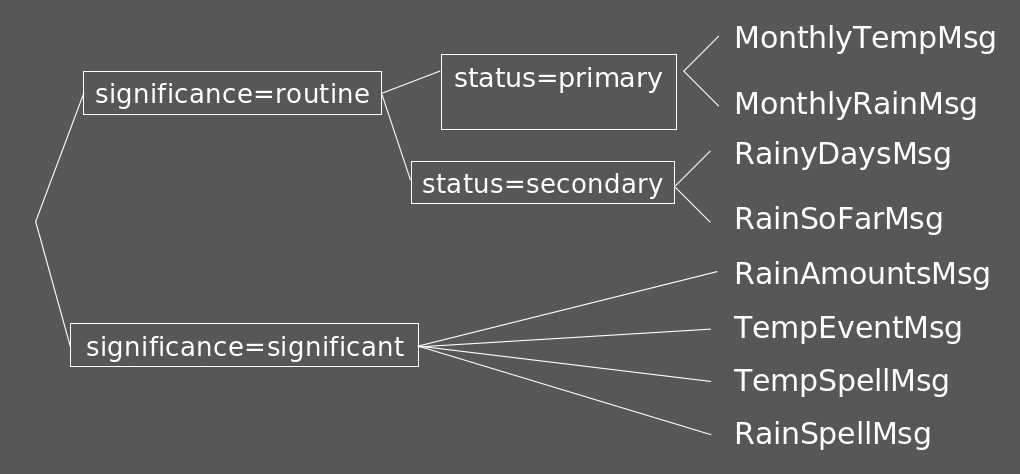
\includegraphics[scale=.4]{pics/pic9.jpg}
\end{center}

\end{frame}

\begin{frame}
\frametitle{Document Structuring en WeatherReporter}

\begin{itemize}
\item SEQUENCE

Dos mensajes pueden conectarse mediante una relaci\'on de SEQUENCE si ambos 
tienen el atributo message-status = primary

\item ELABORATION

Dos mensajes pueden conectarse mediante la relaci\'on ELABORATION si: 
ambos tienen el mismo message-topic, el nucleo tiene menssage-status = primary

\item \ldots
\end{itemize}
\end{frame}

\begin{frame}
\frametitle{Document Structuring en WeatherReporter}

\begin{itemize}

\item Selecionar un mensaje para comenzar con atributo message-significance = routine
\item Aplicar relaciones ret\'oricas a dos mensajes en esta estructura hasta que todos los mensajes hallan sido consumidos o hasta que no puedan aplicarse m\'as relaciones 

\end{itemize}
\end{frame}

\begin{frame}
\frametitle{Ejemplo}

\begin{quote}
The month was cooler and drier than average, with the average number of rain days, but the total rain for the year so far is well below average.  Although there was rain on every day for 8 days from 11th to 18th, rainfall amounts were mostly small.\pause
\end{quote}

\only<2>{
The Message Set:

\ \ \ MonthlyTempMsg (``cooler than average'')\\
\ \ \ MonthlyRainfallMsg (``drier than average'')\\
\ \ \ RainyDaysMsg (``average number of rain days'')\\
\ \ \ RainSoFarMsg (``well below average'')\\
\ \ \ RainSpellMsg (``8 days from 11th to 18th'')\\
\ \ \ RainAmountsMsg (``amounts mostly small'')}\pause

\ \ \ MonthlyTempMsg  -- SEQUENCE $\to$ MonthlyRainfallMsg \pause

\ \ \ MonthlyRainfallMsg -- ELABORATION $\to $ RainyDaysMsg \pause

\ \ \ RainyDaysMsg -- CONTRAST $\to$ RainSoFarMsg\pause

\ \ \ \ldots

\end{frame}

\begin{frame}
\frametitle{Document Planning}

\begin{itemize}
\item El resultado de este paso es un \mH{Plan del Documento}: una estructura en forma de \'arbol
que tiene mensajes en sus nodos terminales.

\item El siguiente paso es realizar estos mensajes como texto
\end{itemize}
 
\end{frame}

\begin{frame}
\frametitle{Temas de Investigaci\'on}

\begin{itemize}
\item Por el momento, la mayor parte del trabajo durante document structuring se hace ad-hoc
\item C\'omo podemos extraer esquemas a partir de un corpus? 
\item Mejor entendimiento de las relaciones ret\'oricas
\item C\'omo podemos integrar esquemas y relaciones ret\'oricas?
\item Knowledge acquisition
\end{itemize}
 
\end{frame}


\end{document}
